\section{Results}
\label{sec:results}
Our study demonstrates the efficacy of our methodology in enhancing the visual presentation of objects within 3D reconstructions. As depicted in Figure 1, the unprocessed Panoptic reconstruction exhibits visual artificats and irregularities, while our approach yields smoothed surfaces, facilitating improved recognition through visual observation. Additionally, we observe the sensitivity of our alignment procedure to the instance masks generated by Panoptic. Although the predicted objects maintain smoothness (likely due to the conditioning in SDFusion), our alignment algorithm occasionally results in object intersection, as illustrated in Figure 2.

\paragraph{Panoptic Reconstruction}

We leverage our synthesized dataset to refine the training of the panoptic reconstruction model proposed by Dahnert et al. \citep{dahnert2021panoptic}.
Initially, we pretrain the 2D encoder, depth estimation and 2D instance prediction with an ADAM optimizer using a batch size of 1 and learning rate 1e-4 for 570k iterations.

The evaluation results for our 2D model compared to the pre-trained model from \citet{dahnert2021panoptic} are presented in \cref{tab:2dresults}.
As depicted in \cref{fig:qual_panoptic}, our approach demonstrates comparable performance to the pre-trained model but still struggles to produce clean depth results, exhibiting certain irregularities.

Despite our efforts, limitations such as time constraints and the relatively small size of our dataset hindered our ability to train a 3D model that achieves performance on par with the pre-trained counterpart. We refer to the future work section in this regard.
\begin{table}
  \centering
  \begin{tabular}{@{}lccc@{}}
    \toprule
     & Depth & Box Class. & Box Regress. \\
    \midrule
    Panoptic & 0.222 & 3.461 & 0.09\\
    Ours & 0.196 & 1.958 & 0.183 \\
    \bottomrule
  \end{tabular}
  \caption{Results for joint training of the 2D encoder, depth estimation and 2D instance prediction. For depth we report the $\ell_1$ distance between the predicted and ground-truth depth maps. Additionally we report the $\ell_1$ distance for the regressed 2D boxes and a CE-loss on the box classification.  }
  \label{tab:2dresults}
\end{table}

\begin{figure}[t]
  \centering
  \begin{subfigure}{0.45\linewidth}
    \centering
    
\includegraphics[width=\linewidth]{figs/depth_ours.png}
    \label{subfig:sub1}
  \end{subfigure}
  \hspace{0.05\linewidth} % Adjust spacing between figures
  \begin{subfigure}{0.45\linewidth}
    \centering
    
\includegraphics[width=\linewidth]{figs/depth_pan.png}
    \label{subfig:sub2}
  \end{subfigure}
  \vspace*{-3mm} % Adjust vertical spacing between the caption and the images
  \caption*{Depth Map}

  \vspace{0.04\linewidth} % Adjust vertical spacing between rows of figures

  \begin{subfigure}{0.45\linewidth}
    \centering
    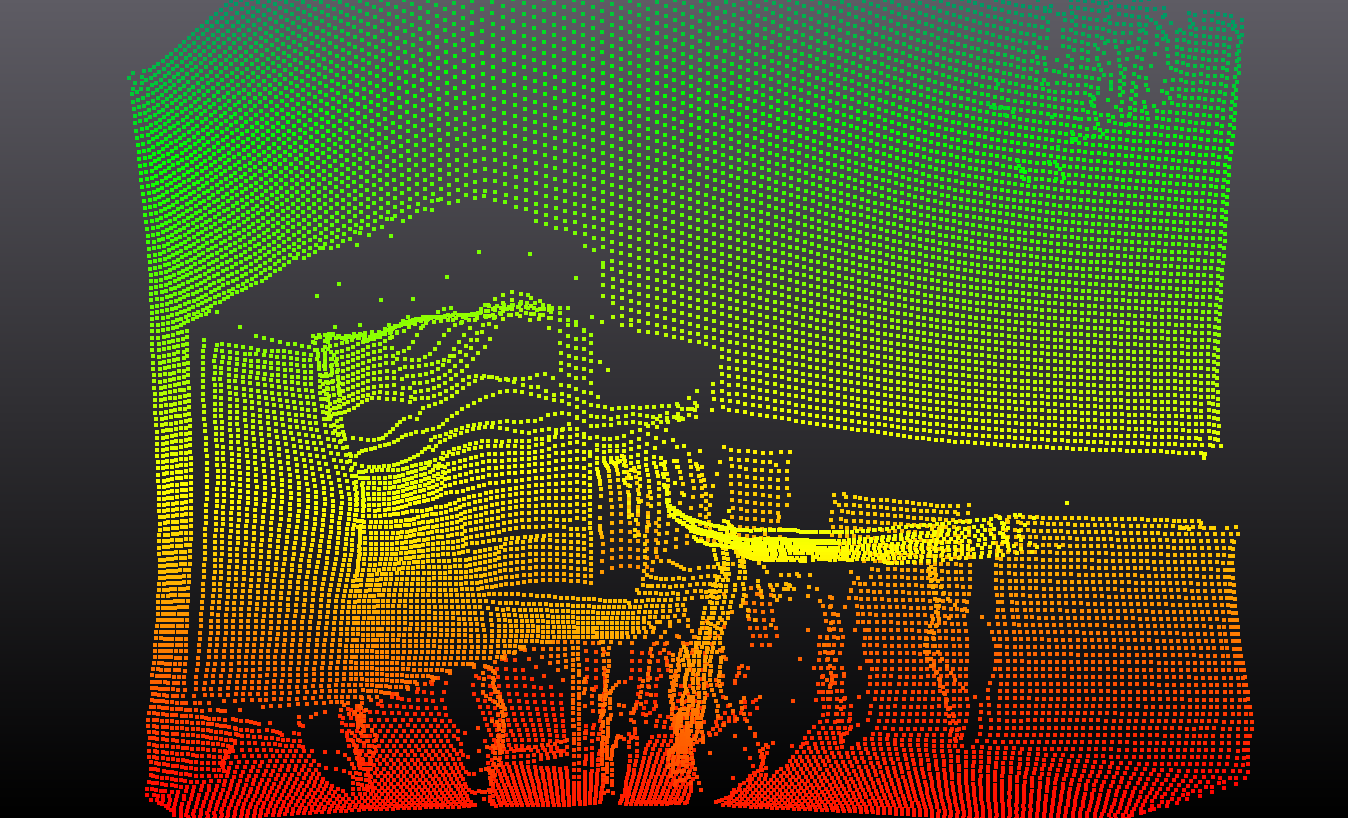
\includegraphics[width=\linewidth]{figs/depthply_ours.png}
    \label{subfig:sub3}
  \end{subfigure}
  \hspace{0.05\linewidth} % Adjust spacing between figures
  \begin{subfigure}{0.45\linewidth}
    \centering
    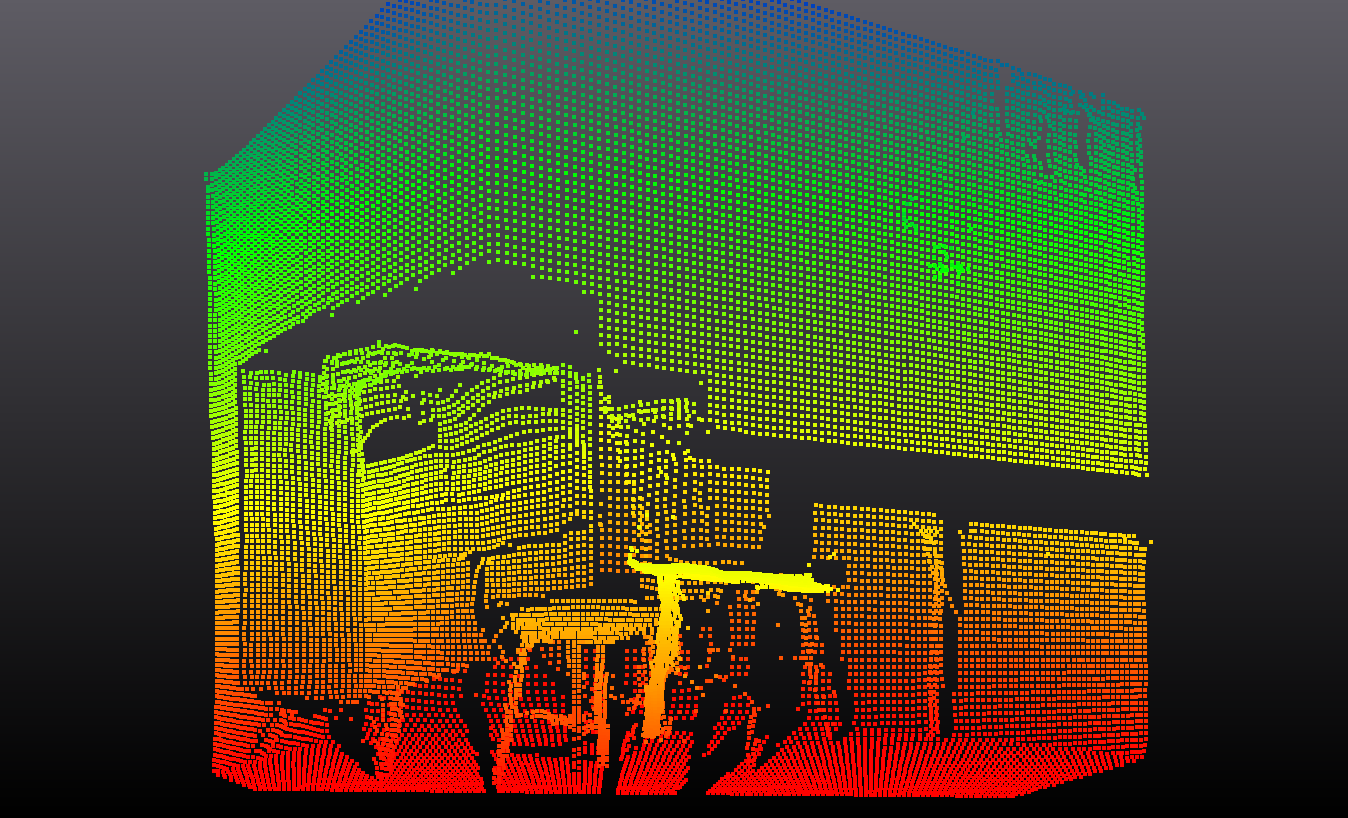
\includegraphics[width=\linewidth]{figs/depthply_pan.png}
    \label{subfig:sub4}
  \end{subfigure}
   \vspace*{-3mm} % Adjust vertical spacing between the caption and the images
   \caption*{Geometry from Depth}

  \caption{2D panoptic results. Ours vs. \citet{dahnert2021panoptic}}
  \label{fig:qual_panoptic}
\end{figure}